\documentclass[12pt]{article}

\usepackage{a4wide,graphicx,amsmath,amssymb,amsfonts,url,psfrag,subcaption}
\usepackage{rotating}
\usepackage{xcolor}
\usepackage{soul}
\usepackage{tikz}
\usepackage{algorithm2e}
\usepackage{todonotes}

\addtolength{\parskip}{3mm}

\usepackage[numbers,sort&compress]{natbib}
\usepackage{lineno, blindtext}
\usepackage[export]{adjustbox}

%\usepackage[dvipsnames]{xcolor}
\definecolor{MyGreen}{HTML}{66C2A5}
\definecolor{MyOrange}{HTML}{FC8D62}
\definecolor{MyBlue}{HTML}{8DA0CB}
\definecolor{MyPink}{HTML}{E78AC3}
\definecolor{MyGreen2}{HTML}{A6D854}
% Notes
\newcommand{\notes}[1]{\textit{\bf[***note -- #1***]}}
\begin{document}







%%%%%%% Figure %%%%%%%%
\newpage
\begin{figure}[htpb]
%
\begin{center}
 \hspace{0.6cm} {$t=0$} \hspace{3.3cm} {$t=50$}  \hspace{3.2cm} {$t=100$} \\
\end{center}
\vspace{-0.9cm}
\begin{center}
\rotatebox[origin=c]{90}{\hspace{0.0cm} Growing Domain \hspace{0.3cm} }
$\vcenter{\hbox{
% L B R T
 \adjincludegraphics[width=4.5cm, trim={{.501\width} 0.0cm 0.0cm {.501\height}}, clip]{Figs/Snapshots/EllipticGrowingConvergence/snapshot0}
\adjincludegraphics[width=4.5cm, trim={{.501\width} 0.0cm 0.0cm {.501\height}}, clip]{Figs/Snapshots/EllipticGrowingConvergence/snapshot50}
\adjincludegraphics[width=4.5cm, trim={{.501\width} 0.0cm 0.0cm {.501\height}}, clip]{Figs/Snapshots/EllipticGrowingConvergence/snapshot100}
}}$
\end{center}

\vspace{-0.9cm}

\begin{center}
\rotatebox[origin=c]{90}{\hspace{0.0cm} Box Domain (Mesh BC) \hspace{0.3cm} }
$\vcenter{\hbox{
% L B R T
 \adjincludegraphics[width=4.5cm, trim={ 0.0cm 0.0cm {.501\width} {.501\height}}, clip]{Figs/Snapshots/EllipticGrowingConvergence/snapshot0}
  \adjincludegraphics[width=4.5cm, trim={ 0.0cm 0.0cm {.501\width} {.501\height}}, clip]{Figs/Snapshots/EllipticGrowingConvergence/snapshot50}
 \adjincludegraphics[width=4.5cm, trim={ 0.0cm 0.0cm {.501\width} {.501\height}}, clip]{Figs/Snapshots/EllipticGrowingConvergence/snapshot100}
}}$
\end{center}

\vspace{-0.9cm}

\begin{center}
\rotatebox[origin=c]{90}{\hspace{0.0cm} Box Domain (Tissue BC) \hspace{0.3cm} }
$\vcenter{\hbox{
% L B R T
 \adjincludegraphics[width=4.5cm, trim={0.0cm {.501\height} {.501\width} 0.0cm}, clip]{Figs/Snapshots/EllipticGrowingConvergence/snapshot0}
  \adjincludegraphics[width=4.5cm, trim={0.0cm {.501\height} {.501\width} 0.0cm}, clip]{Figs/Snapshots/EllipticGrowingConvergence/snapshot50}
 \adjincludegraphics[width=4.5cm, trim={0.0cm {.501\height} {.501\width} 0.0cm}, clip]{Figs/Snapshots/EllipticGrowingConvergence/snapshot100}
}}$
\end{center}

\vspace{-0.9cm}

\begin{center}
\rotatebox[origin=c]{90}{\hspace{0.0cm} Box Domain (Box BC) \hspace{0.3cm} }
$\vcenter{\hbox{
% L B R T
 \adjincludegraphics[width=4.5cm, trim={{.501\width} {.501\height} 0.0cm 0.0cm}, clip]{Figs/Snapshots/EllipticGrowingConvergence/snapshot0}
\adjincludegraphics[width=4.5cm, trim={{.501\width} {.501\height} 0.0cm 0.0cm}, clip]{Figs/Snapshots/EllipticGrowingConvergence/snapshot50}
\adjincludegraphics[width=4.5cm, trim={{.501\width} {.501\height} 0.0cm 0.0cm}, clip]{Figs/Snapshots/EllipticGrowingConvergence/snapshot100}
}}$
\end{center}



\vspace{-0.5cm}
\caption{{\bf Convergence of Elliptic PDE solutions.} 
	Nutirent dependenent CCM. Convergence as space step is decreased. Dashes line is results from solving the PDE on a growing domain. }
\label{fig:2druntime}
\end{figure}

%%%%%%% Figure %%%%%%%%
\newpage
\begin{figure}[htpb]
%
\begin{center}
 \hspace{0.6cm} {$t=0$} \hspace{3.3cm} {$t=50$}  \hspace{3.2cm} {$t=100$} \\
\end{center}
\vspace{-0.9cm}

\begin{center}
\rotatebox[origin=c]{90}{\hspace{0.0cm} Box Domain (Mesh BC) \hspace{0.3cm} }
$\vcenter{\hbox{
% L B R T
 \adjincludegraphics[width=4.5cm, trim={ 0.0cm 0.0cm {.501\width} {.501\height}}, clip]{Figs/Snapshots/EllipticGrowingConvergence/snapshotFine0}
  \adjincludegraphics[width=4.5cm, trim={ 0.0cm 0.0cm {.501\width} {.501\height}}, clip]{Figs/Snapshots/EllipticGrowingConvergence/snapshotFine50}
 \adjincludegraphics[width=4.5cm, trim={ 0.0cm 0.0cm {.501\width} {.501\height}}, clip]{Figs/Snapshots/EllipticGrowingConvergence/snapshotFine100}
}}$
\end{center}

\vspace{-0.9cm}

\begin{center}
\rotatebox[origin=c]{90}{\hspace{0.0cm} Box Domain (Tissue BC) \hspace{0.3cm} }
$\vcenter{\hbox{
% L B R T
 \adjincludegraphics[width=4.5cm, trim={0.0cm {.501\height} {.501\width} 0.0cm}, clip]{Figs/Snapshots/EllipticGrowingConvergence/snapshotFine0}
  \adjincludegraphics[width=4.5cm, trim={0.0cm {.501\height} {.501\width} 0.0cm}, clip]{Figs/Snapshots/EllipticGrowingConvergence/snapshotFine50}
 \adjincludegraphics[width=4.5cm, trim={0.0cm {.501\height} {.501\width} 0.0cm}, clip]{Figs/Snapshots/EllipticGrowingConvergence/snapshotFine100}
}}$
\end{center}

\vspace{-0.9cm}
\begin{center}
 \hspace{0.6cm} {Mesh BC} \hspace{3.3cm} {Tissue BC}  \\
\end{center}
\vspace{-0.9cm}
\begin{center}
\rotatebox[origin=c]{90}{\hspace{0.0cm} Box Domain \hspace{0.3cm} }
$\vcenter{\hbox{
% L B R T
 \adjincludegraphics[width=4.5cm, trim={0.0cm 0.0cm 0.0cm 10.0cm}, clip]{Figs/Snapshots/MeshBcExample}
 \adjincludegraphics[width=4.5cm, trim={0.0cm 5.0cm 0.0cm 5.0cm}, clip]{Figs/Snapshots/TissueBcExample}
}}$


\end{center}



\vspace{-0.5cm}
\caption{{\bf Convergence of Elliptic PDE solutions.} 
	Nutirent dependenent CCM. Convergence as space step is decreased. Dashes line is results from solving the PDE on a growing domain. }
\label{fig:2druntime}
\end{figure}


%%%%%%% Figure %%%%%%%%
\newpage
\begin{figure}[htpb]
%
\begin{center}
 \hspace{1.5cm} {All Cells} \hspace{3.1cm} {Proliferating Cells} \\
\end{center}
\vspace{-0.9cm}
\begin{center}
\rotatebox[origin=c]{90}{\hspace{0.0cm} Box BC \hspace{0.3cm} }
$\vcenter{\hbox{
\begin{tikzpicture}
    \node[anchor=south west,inner sep=0] (image) at (0,0) {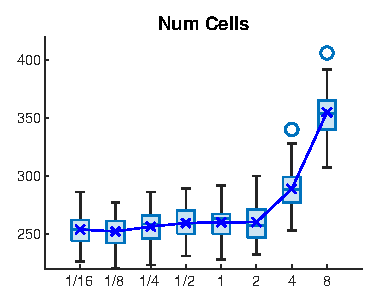
\includegraphics[width=5.5cm, trim={0.0cm 0.0cm 0.0cm 0.0cm}, clip]{Figs/CellNumBox_EllipticConvergenceGrowingTissueBoxDomainBoxBcVolumeScaledAveragedPde}};
    %L B R T
%    \node[anchor=south west,inner sep=0] (image) at (2.95,2.55) {\includegraphics[width=1.5cm, trim={4.6cm 2.3cm 0.4cm 1.9cm}, clip]{Figs/2d_mesh/explicitLegend}};
    \end{tikzpicture}
    %
\begin{tikzpicture}
    \node[anchor=south west,inner sep=0] (image) at (0,0) {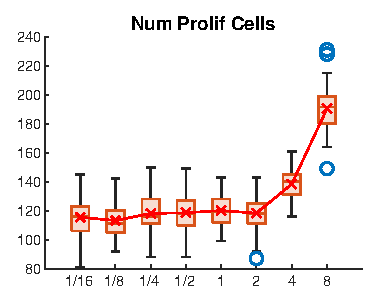
\includegraphics[width=5.5cm, trim={0.0cm 0.0cm 0.0cm 0.0cm}, clip]{Figs/ProlifCellNumBox_EllipticConvergenceGrowingTissueBoxDomainBoxBcVolumeScaledAveragedPde}};
    %L B R T
%    \node[anchor=south west,inner sep=0] (image) at (2.95,2.55)  {\includegraphics[width=1.5cm, trim={4.6cm 2.3cm 0.4cm 1.9cm}, clip]{Figs/2d_mesh/explicitLegend}};
\end{tikzpicture}}}$
\end{center}
\begin{center}
 \hspace{1.5cm} {All Cells} \hspace{3.1cm} {Proliferating Cells} \\
\end{center}
\vspace{-0.9cm}
\begin{center}
\rotatebox[origin=c]{90}{\hspace{0.0cm} Tissue BC \hspace{0.3cm} }
$\vcenter{\hbox{
\begin{tikzpicture}
    \node[anchor=south west,inner sep=0] (image) at (0,0) {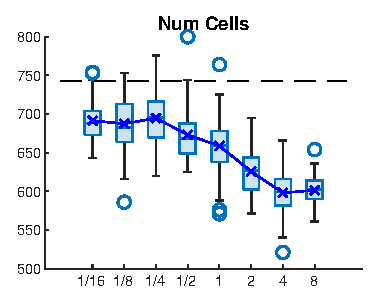
\includegraphics[width=5.5cm, trim={0.0cm 0.0cm 0.0cm 0.0cm}, clip]{Figs/CellNumBox_EllipticConvergenceGrowingTissueBoxDomainTissueBcVolumeScaledAveragedPde}};
    %L B R T
%    \node[anchor=south west,inner sep=0] (image) at (2.95,2.55) {\includegraphics[width=1.5cm, trim={4.6cm 2.3cm 0.4cm 1.9cm}, clip]{Figs/2d_mesh/explicitLegend}};
    \end{tikzpicture}
    %
\begin{tikzpicture}
    \node[anchor=south west,inner sep=0] (image) at (0,0) {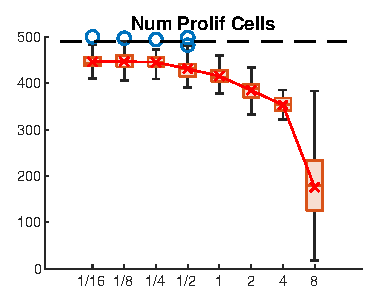
\includegraphics[width=5.5cm, trim={0.0cm 0.0cm 0.0cm 0.0cm}, clip]{Figs/ProlifCellNumBox_EllipticConvergenceGrowingTissueBoxDomainTissueBcVolumeScaledAveragedPde}};
    %L B R T
%    \node[anchor=south west,inner sep=0] (image) at (2.95,2.55)  {\includegraphics[width=1.5cm, trim={4.6cm 2.3cm 0.4cm 1.9cm}, clip]{Figs/2d_mesh/explicitLegend}};
\end{tikzpicture}}}$
\end{center}
\begin{center}
 \hspace{1.5cm} {All Cells} \hspace{3.1cm} {Proliferating Cells} \\
\end{center}
\vspace{-0.9cm}
\begin{center}
\rotatebox[origin=c]{90}{\hspace{0.0cm} Mesh BC \hspace{0.3cm} }
$\vcenter{\hbox{
\begin{tikzpicture}
    \node[anchor=south west,inner sep=0] (image) at (0,0) {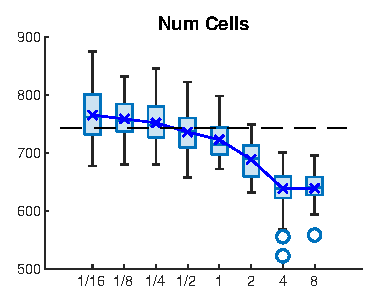
\includegraphics[width=5.5cm, trim={0.0cm 0.0cm 0.0cm 0.0cm}, clip]{Figs/CellNumBox_EllipticConvergenceGrowingTissueBoxDomainMeshBcVolumeScaledAveragedPde}};
    %L B R T
%    \node[anchor=south west,inner sep=0] (image) at (2.95,2.55) {\includegraphics[width=1.5cm, trim={4.6cm 2.3cm 0.4cm 1.9cm}, clip]{Figs/2d_mesh/explicitLegend}};
    \end{tikzpicture}
    %
\begin{tikzpicture}
    \node[anchor=south west,inner sep=0] (image) at (0,0) {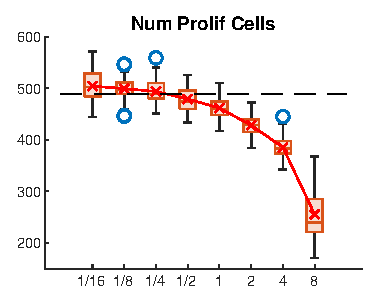
\includegraphics[width=5.5cm, trim={0.0cm 0.0cm 0.0cm 0.0cm}, clip]{Figs/ProlifCellNumBox_EllipticConvergenceGrowingTissueBoxDomainMeshBcVolumeScaledAveragedPde}};
    %L B R T
%    \node[anchor=south west,inner sep=0] (image) at (2.95,2.55)  {\includegraphics[width=1.5cm, trim={4.6cm 2.3cm 0.4cm 1.9cm}, clip]{Figs/2d_mesh/explicitLegend}};
\end{tikzpicture}}}$
\end{center}

%\vspace{-0.8cm}
%\begin{center}
% \hspace{0.1cm} { 2D VD} \hspace{2.8cm} { 3D OS} \\
%\end{center}
%\vspace{-0.9cm}
%%(b)
%%\vspace{-0.5cm}
%\begin{center}
%$\vcenter{\hbox{
%\begin{tikzpicture}
%    \node[anchor=south west,inner sep=0] (image) at (0,0) {\includegraphics[width=4.6cm, trim={0.075cm 0.1cm 0.49cm 0.24cm}, clip]{Figs/2d_vertex/AMT_1_ComputationalTime}};
%    %L B R T
%   % \node[anchor=south west,inner sep=0] (image) at (2.95,2.55) {\includegraphics[width=1.5cm, trim={4.6cm 2.3cm 0.4cm 1.9cm}, clip]{Figs/2d_mesh/explicitLegend}};
%\end{tikzpicture}
%%
%\begin{tikzpicture}
%    \node[anchor=south west,inner sep=0] (image) at (0,0) {\includegraphics[width=4.6cm, trim={0.075cm 0.1cm 0.49cm 0.24cm}, clip]{Figs/3d_node/step_51_AMT_1_ComputationalTime}};
%    %L B R T
%    %\node[anchor=south west,inner sep=0] (image) at (2.95,2.55) {\includegraphics[width=1.5cm, trim={4.6cm 2.3cm 0.4cm 1.9cm}, clip]{Figs/2d_mesh/explicitLegend}};
%    \end{tikzpicture}}}$
%\end{center}
\vspace{-0.5cm}
\caption{{\bf Convergence of Elliptic PDE solutions.} 
	Nutirent dependenent CCM. Convergence as space step is decreased. Dashes line is results from solving the PDE on a growing domain. }
\label{fig:2druntime}
\end{figure}


%%%%%%% Figure %%%%%%%%
\newpage
\begin{figure}[htpb]
%
\begin{center}

\begin{tikzpicture}
    \node[anchor=south west,inner sep=0] (image) at (0,0) {
\includegraphics[width=10cm, trim={0.0cm 0.0cm 0.0cm 0.0cm}, clip]{Figs/Boundary_EllipticConvergenceGrowingTissueBoxDomainBoxBcVolumeScaledAveragedPde}};
    %L B R T
%    \node[anchor=south west,inner sep=0] (image) at (2.95,2.55) {\includegraphics[width=1.5cm, trim={4.6cm 2.3cm 0.4cm 1.9cm}, clip]{Figs/2d_mesh/explicitLegend}};
    \end{tikzpicture}
\end{center}
\begin{center}
\rotatebox[origin=c]{90}{\hspace{0.0cm} Box BC \hspace{0.3cm} }
$\vcenter{\hbox{
\begin{tikzpicture}
    \node[anchor=south west,inner sep=0] (image) at (0,0) {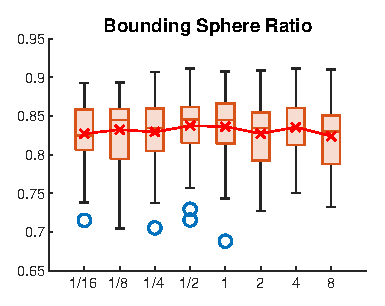
\includegraphics[width=5.5cm, trim={0.0cm 0.0cm 0.0cm 0.0cm}, clip]{Figs/BoundingSphereRatioBox_EllipticConvergenceGrowingTissueBoxDomainBoxBcVolumeScaledAveragedPde}};
    %L B R T
%    \node[anchor=south west,inner sep=0] (image) at (2.95,2.55) {\includegraphics[width=1.5cm, trim={4.6cm 2.3cm 0.4cm 1.9cm}, clip]{Figs/2d_mesh/explicitLegend}};
    \end{tikzpicture}
    %
\begin{tikzpicture}
    \node[anchor=south west,inner sep=0] (image) at (0,0) {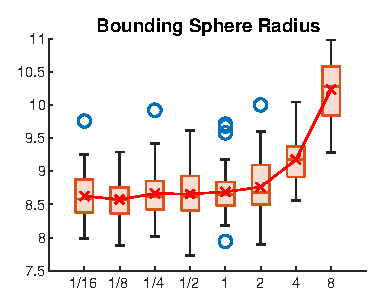
\includegraphics[width=5.5cm, trim={0.0cm 0.0cm 0.0cm 0.0cm}, clip]{Figs/BoundingSphereBox_EllipticConvergenceGrowingTissueBoxDomainBoxBcVolumeScaledAveragedPde}};
    %L B R T
%    \node[anchor=south west,inner sep=0] (image) at (2.95,2.55)  {\includegraphics[width=1.5cm, trim={4.6cm 2.3cm 0.4cm 1.9cm}, clip]{Figs/2d_mesh/explicitLegend}};
\end{tikzpicture}}}$
\end{center}
\caption{{\bf Convergence of Elliptic PDE solutions.} 
	Nutirent dependenent CCM. Convergence as space step is decreased. Dashes line is results from solving the PDE on a growing domain. }
\label{fig:2druntime}
\end{figure}


\end{document}
